% last updated in April 2002 by Antje Endemann
% Based on CVPR 07 and LNCS, with modifications by DAF, AZ and elle, 2008 and AA, 2010, and CC, 2011; TT, 2014; AAS, 2016

\documentclass[runningheads]{llncs}
\usepackage{graphicx}
\usepackage{amsmath,amssymb} % define this before the line numbering.
\usepackage{algorithm}
\usepackage{algpseudocode}
\usepackage{ruler}
\usepackage{color}
\usepackage[width=122mm,left=12mm,paperwidth=146mm,height=193mm,top=12mm,paperheight=217mm]{geometry}
\begin{document}
% \renewcommand\thelinenumber{\color[rgb]{0.2,0.5,0.8}\normalfont\sffamily\scriptsize\arabic{linenumber}\color[rgb]{0,0,0}}
% \renewcommand\makeLineNumber {\hss\thelinenumber\ \hspace{6mm} \rlap{\hskip\textwidth\ \hspace{6.5mm}\thelinenumber}}
% \linenumbers
\pagestyle{headings}
\mainmatter
\def\ECCV16SubNumber{***}  % Insert your submission number here

\title{Unsupervised Deep Domain Adaptation on People Detection} % Replace with your title

\titlerunning{ECCV-16 submission ID \ECCV16SubNumber}

\authorrunning{ECCV-16 submission ID \ECCV16SubNumber}

\author{Anonymous ECCV submission}
\institute{Paper ID \ECCV16SubNumber}


\maketitle

\begin{abstract}
This paper addresses the problem of unsupervised domain adaptation on the task of people detection in crowded scenes. That is, given a well-trained deep detection model on source domain, we aim to adapt it into the target domain for which no annotations are needed. Firstly, we utilize iterative algorithm to auto-annotate samples on target domain. While auto-annotated samples include noise, the rate of false positive tends to explored. Thus, we mixed into training examples from source domain to suppress the data noise. Furthermore, we transform the inner product layers of our network into two separate layers and proposed a weights regularizer to avoid overfitting. Compared to generic model without any fine tuning on samples on target domain, the proposed method increased recall by $xx\%$ with precision drop from $xx\%$ to $xx\%$ on the target scenes. Also, we perform our algorithm on standard domain adaptation benchmarks Office Dataset with both supervised and unsupervised settings and our results are state of art.

\keywords{Unsupervised Domain Adaptation, Deep Neural Network, People Detection}
\end{abstract}


\section{Introduction}

Deep neural network has outstanding result on computer vision tasks, however, it require large labelled dataset. In famous challenges like PASCAL VOC and MS COCO, over millions of images with labels are needed for training. In surveillance applications like people detection, the annotation process is even human resource consuming. Till today, there are millions of cameras deployed for surveillance. However, surveillance situations varies in background, lights, viewpoints and so on in real world, which make the labelling work for all surveillance applications ever more unpractice. In the task of people detection, tens of thousands of annotated images are needed to train a deep neural network.
\par
When labelled data are few and even lack of in target domain, domain adaptation help to reduce the amount of labelled data needed when given abundant labelled data in source domain. Most traditional works \cite{saenko2010adapting,kulis2011you,gopalan2011domain,huang2006correcting,gretton2009covariate} try to learn a shared representation between source and target domain, or project features into a common subspace. Recently, works are also \cite{wang2014scene,zeng2014deep,hattori2015learning} proposed to learn scene-specific detector by deep architectures. In our task of people detection, we try to shift deep detection network well-trained on the source scene to target scenes on which no annotation are needed.
\par
In this paper, we proposed a new approach of unsupervised deep domain adaptation on people detection. Using generic model as initialization, we firstly use iterative algorithm to auto-annotate samples on target domain as fake ground truth. During every iteration, target model are updated and utilized to auto-annotate samples for next iteration. However, the data noise in auto-annotated dataset, like lack of true negative instances and false positive instances, will leads to exploration of false positive rate, as well as impeding further increase of recall. In order to eliminate the effect of data noise, two methods are proposed to regularize the training of the deep network. On the one hand, we mixed into auto-annotated dataset with annotated samples from source domain to compensate the lack of true negative instances. On the other hand, we separate the operation of last inner product layer of our network into two sub-operations -- element-wise multiply and sum operations, resulting new element-wise multiply layer and sum layer. Thus, a weights regularizer on element-wise layer can be added into the deep network as unsupervised loss to avoid exploration of false positive rate and boost recall.
\par
Also, we further evaluate our method on standard domain adaptation benchmark Office Dataset. The results of our adaptation approach outperform previously published works on both supervised and unsupervised settings, which demonstrate the feasibility of our adaptation approach on both detection and classification tasks.
\par
The contributions of our work are three folds.
\begin{itemize}
\item We provided a feasible scheme to shift deep detection network well-trained on the source scene to target scenes on which no annotated data are needed. This makes easier the widely deploy of deep neural network on various surveillance applications.
\item As most algorithms focus on the last feature vector (also last inner product layer), we have one step further and transform the last inner product layer into element-wise multiply layer and sum layer. A weight regularizer can, thus, be added on element-wise layer to have better effect on suppressing exploration of false positive rate and increasing recall.
\item Experiments on standard domain adaptation benchmarks also demonstrate the effectiveness of our approach on other deep domain adaptation tasks.
\end{itemize}

The remainder of this paper is organized as follows. Section \ref{section:Relate Work} reviews related works. Section \ref{section:Our Approach} presents the details of our approach. Experimental results are shown in Section \ref{section:Experiment Results}. Section \ref{section:Conclusions} concludes the paper.

\section{Relate Work}
\label{section:Relate Work}
\par
In many detection works, generic model trained by large amount of samples on source domain are directly utilized to detect on target domain. They assume that samples on target domain are subsets of source domain. However, when the distribution of data on target and source domain varies largely, the performance will drop significantly. Domain adaptation aims to reduce the amount of data needed for target domain.

Many domain adaptation works tried to learn a common representation space shared between source and target domain. Saenko et al. \cite{saenko2010adapting,kulis2011you} proposed a both linear-transform-based technique and kernel-transform-based technique to minimize domain changes. Gopalan et al. \cite{gopalan2011domain} projected features into Grassmann manifold instead of operating on features of raw data. Alternatively, Mesnil et al. \cite{mesnil2012unsupervised} used transfer learning to obtain good representations. However, these methods are limited because scene-specific features are not learned to boost accuracy. The regularizer of our method are inspired these works.

Another group of works \cite{huang2006correcting,gretton2009covariate,gong2013connecting} on domain adaptation is to make the distribution of source and target domain more similar. Among these works, Maximum Mean Discrepancy (MMD) is used to as a metric to reselect samples from source domain in order to have similar distribution as target samples. In \cite{ghifary2014domain}, MMD is incorporated as regularization to reduce distribution mismatch.

There are also works on deep adaptation to construct scene-specific detector. Wang et al.\cite{wang2014scene} explored context cues to compute confidence, and \cite{zeng2014deep} learns distributions of target samples and proposed a cluster layer for scene-specific visual patterns. These works reweighted auto-annotated samples for their final object function and additional context cues are needed for reliable performance. Alternately, Hattori el al. \cite{hattori2015learning} learned scene-specific detector by generating a spatially-varying pedestrian appearance model. And Pishchulin et al. \cite{pishchulin2011learning} used 3D shape models to generate training data. However, Synthesis for domain adaptation are also costly.

\section{Our Approach}
\label{section:Our Approach}

In this section, we introduce our unsupervised deep domain adaptation approach on the task of people detection. We denote the training images of source domain as  ${\bf X}^{S} = \{x^{S}_{i}\}^{N^{S}}_{i=1}$ and that of target domain as ${\bf X}^{T} = \{x^{T}_{j}\}^{N^{T}}_{j=1}$. For each image in source domain, we have corresponding annotations denoted as ${\bf B}^{S}_{i} = \{b^{S}_{i,k}\}^{N^{S}_{i}}_{k=1}$ with $b^{S}_{i,k} = (x,y,w,h) \in R^{4}$, however, the annotations for images in target domain are auto-labelled which we denote as ${\bf \tilde{B}}^{T}_{j} = \{\tilde{b}^{T}_{j,k}\}^{N^{T}_{j}}_{k=1}$ with $\tilde{b}^{T}_{j,k} = (\tilde{x},\tilde{y},\tilde{w},\tilde{h}) \in R^{4}$. The annotations for target domain changes for every iteration during the adaptation process. Human annotated images on target domain are used only for evaluation.

The adaptation architecture of our approach consists of two streams -- source stream $M^{S}$ and target stream $M^{T}$, as shown in Fig x(!). Source stream takes samples from source domain as input, and target stream operates on samples from target domain. These two streams can utilize any end to end deep detection network as their model. Here we use the below mentioned network in Sec \ref{section:Detection Network} in our experiment. In initialization stage, we firstly use abundant annotated samples from source domain to train the model of source stream under a supervised loss function to regress bounding box. After its convergence, the weights of the model of source stream are used to initialize target stream. In adaptation stage, iteration algorithm is used as training method. Target model in target stream is trained and upgraded in this process while source stream stays static.

Both supervised loss and unsupervised regularizer are designed as loss function to train the target stream for learning scene-specific detector as well as avoid overfitting. For supervised loss, the auto-annotated data can be used as training labels. As the auto-annotated samples contains data error, an unsupervised loss are required to regularize the network. We take the source model in source stream as a reference for feature vector distribution. We defined the combination of supervised loss and unsupervised loss as our loss function for adaptation:
\begin{eqnarray}
% \nonumber to remove numbering (before each equation)
  L(\theta^{T}|{\bf X}^{S},{\bf B}^{S},{\bf X}^{T},{\bf \tilde{B}}^{T},\theta^{S}) &=& L_{S} + \alpha * L_{U} \\
  L_{S} &=&  \sum^{N^{T}}_{j=1}{\sum^{N^{T}_{J}}_{k=1}( r(\theta^{T}|x^{T}_{j},\tilde{b}^{T}_{j,k})+c(\theta^{T}|x^{T}_{j},\tilde{b}^{T}_{j,k}) )} \\
  L_{U} &=& L_{MMD}(\theta^{T}|{\bf X}^{S},{\bf X}^{T},\theta^{S}) \label{Eq:lmmd}
\end{eqnarray}
where $L_{S}$ is supervised loss to learn the scene-specific detector and $L_{U}$ is the unsupervised regularizer part. $r(\cdot)$ is a regression loss for bounding box location, like norm-1 loss, and $c(\cdot)$ is a classification loss for bounding box confidence, such as cross-entropy loss. And $L_{MMD}(\cdot)$ is the MMD-based loss for unsupervised regularization. Coefficient $\alpha$ balance the effect of supervised and unsupervised loss. We set $\alpha = 10$ in our experiments.

\begin{figure}
\centering
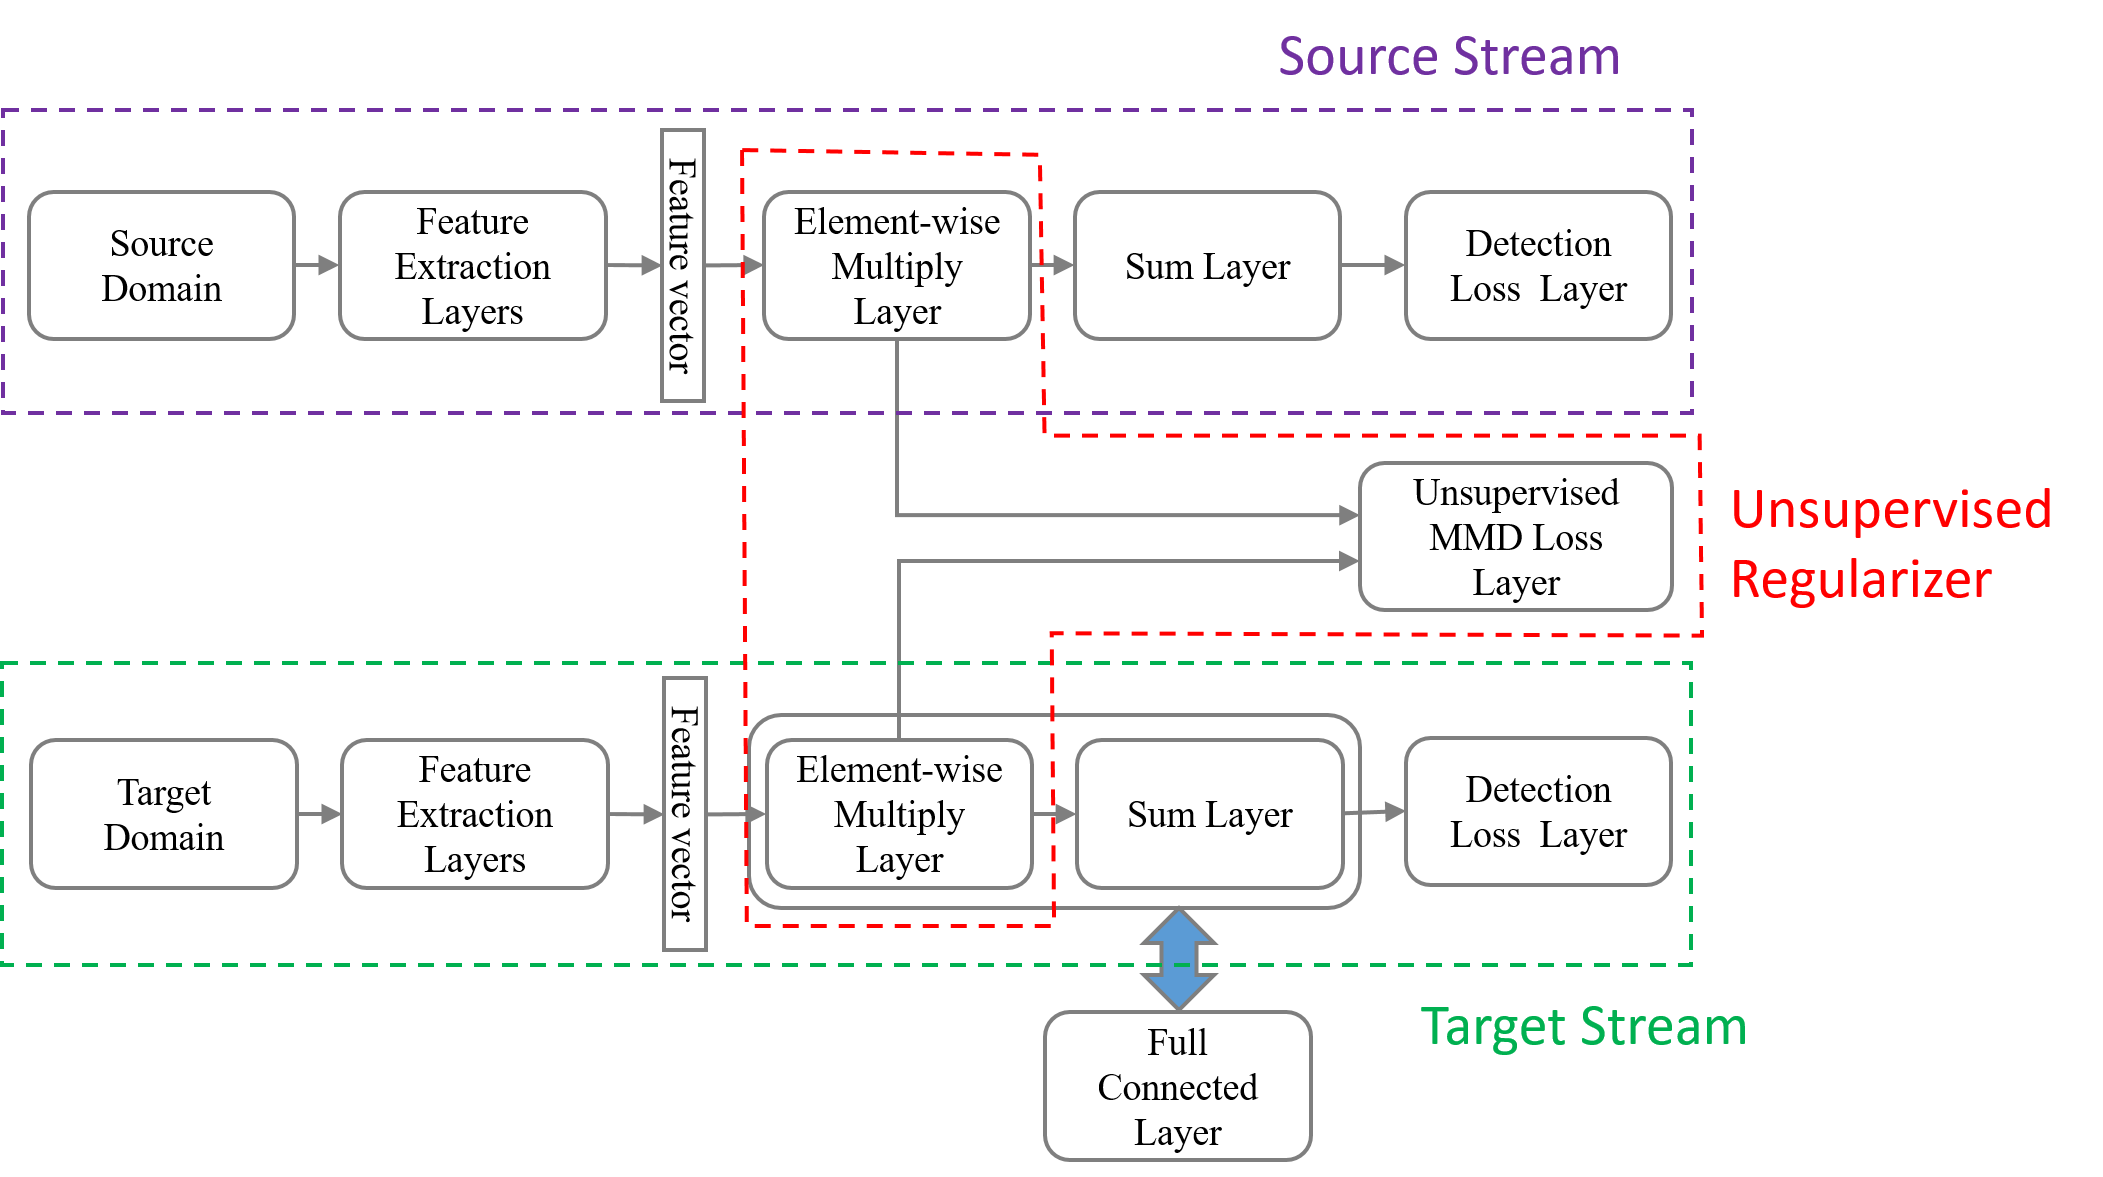
\includegraphics[height=4.5cm]{images/streams.png}
\caption{One kernel at $x_s$ ({\it dotted kernel}) or two kernels at
$x_i$ and $x_j$ ({\it left and right}) lead to the same summed estimate
at $x_s$. This shows a figure consisting of different types of
lines. Elements of the figure described in the caption should be set in
italics,
in parentheses, as shown in this sample caption. The last
sentence of a figure caption should generally end without a full stop}
\label{fig:example}
\end{figure}

\subsection{Detection Network}
\label{section:Detection Network}
The generic model \footnote{Proposed by Russel et al.} used in our adaptation architecture for source and target stream is an end to end detection network without any precomputed region proposals needed. It consists of a GoogLeNet \cite{szegedy2015going} for feature extraction and a RNN-based decoder for output of bounding box and corresponding confidence, as shown in Fig x(!). Firstly, the GoogLeNet model encode the image into a feature map (15x20x1024) of which each 1024 dimension vector are data representation of its receptive field corresponding to a subregion of the image. Then the RNN-based layers with batch size 300 will decode the data representation and sequentially predict 5 possible bounding boxes by the order of its corresponding confidence. Finally, all outputs are summarized to give final detection results. When trained with abundant samples from source domain, the obtained model has a high precision on target domain, however, its recall is low. Also, different from other detection network \cite{girshick2015fast,vu2015context}, which need precomputed proposals for classification and fine regression, this generic model directly predict bounding boxes with high confidence. Thus, negative instances may contain people and non-people predictions, and cannot be employed in adaptation training.

\begin{figure}
\centering
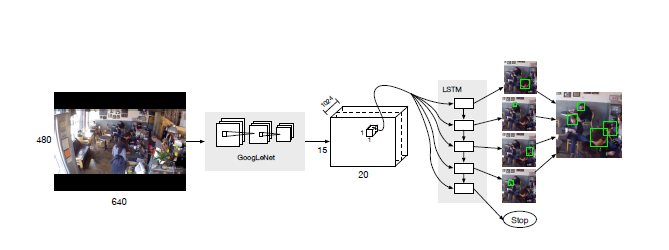
\includegraphics[height=4.5cm]{images/dummyimage.png}
\caption{One kernel at $x_s$ ({\it dotted kernel}) or two kernels at
$x_i$ and $x_j$ ({\it left and right}) lead to the same summed estimate
at $x_s$. This shows a figure consisting of different types of
lines. Elements of the figure described in the caption should be set in
italics,
in parentheses, as shown in this sample caption. The last
sentence of a figure caption should generally end without a full stop}
\label{fig:example}
\end{figure}

\subsection{Iterative Algorithm}
\label{Section:Iterative Algorithm}
In this section we introduce the iteration algorithm as training method at adaptation stage. The auto-annotating tool takes images on target domain with high confidence as training data for next iteration. To generate the auto-annotated data for the first iteration, we utilize the generic model well-trained on source domain, which results in training set on the target domain. As mentioned in Sec \ref{section:Detection Network}, the training set on target domain auto-annotated by the generic model in our experiment have low recall and high precision. At subsequent iterations, training set on target domain are auto-annotated by upgraded model resulting from training of last iteration. Among every iteration, these auto-annotated data are used as training data to upgrade the deep network.

As the training set on target domain auto-annotated for the training of first iteration have low recall rate and people and non-people regions mixed in negative instances, we ignore back propagation of bounding boxes with low confidence during training. That is, we encourage the network to have more confidence on positive instances and stay conservative toward negative instances. This policy will no doubt resulting predictions of many non-people instance and impeding the further training when many non-people instances are regarded as people instances by the target model. To compensate for lack of true negative instances, we add annotated samples from source domain into the training data, which are human annotated and can thus provide true negative samples. In our experiment, when training on additional samples from source domain, we only do back propagation of bounding boxes with low confidence. At the same time, the unsupervised loss will also regularize the network. The complete adaptation process is illustrated in Algorithm \ref{algorithm:Deep domain adaptation algorithm (to be completed)}. After a predetermined iteration limit $N^{I}$ is reached, we obtain our final detection model on the target domain.

\begin{algorithm}
\caption{Deep domain adaptation algorithm (to be completed)}
\label{algorithm:Deep domain adaptation algorithm (to be completed)}
\begin{algorithmic}[1]
\Procedure{Deep domain adaptation} {} \\
\indent Train source model on source stream with abundant annotated data \\
\indent Use well-trained source model on source stream to initialize model on target stream as $M_{0}$
\For{i = 0:$N^{I}$} \\
\indent \indent $M_{i}$ generate "fake ground truth" Gi of target domain \\
\indent \indent balbal \\
\indent \indent balbabla \\
\indent \indent Gi = Gi + random samples from source domain \\
\indent \indent Take Gi as training data to upgrade $M_{i}$ into $M_{i+1}$
\EndFor \\
\indent $M_{N^{I}}$: final model.
\EndProcedure
\end{algorithmic}
\end{algorithm}


\subsection{Unsupervised weights regularizer on Element-wise Multiply Layer}

\subsubsection{Element-wise Multiply Layer}
\label{section:Element-wise Multiply Layer}
In deep neural network, the last feature vector layer are taken as an important data representation of input images. However, in this paper, we take one step further to focus on the last full connected layer which serves as an decoder to decode rich information contained in the last feature vector into final outputs. As source model are trained with abundant labelled data on source domain, the parameters of the last full connected layer are also well converged. We assume that a regularizer on the last full connected layer will achieve better results compared with the last feature vector layer. Firstly, denote the last feature vector, parameters of the last full connected layer and final outputs as ${\bf F}_{(N^{B}\times N^{D})}$, ${\bf C}_{(N^{D}\times N^{O})}$ and ${\bf P}_{(N^{B}\times N^{O})}$, respectively. The operation of full connected layer can be thus formulated as matrix multiply:
\begin{eqnarray}
% \nonumber to remove numbering (before each equation)
  {\bf P} &=& {\bf F}*{\bf C} \\
  P_{b,o} &=&  \sum_{d}{F_{b,d}*K_{d,o}}
\end{eqnarray}
Inspired by this form, we separate the above formula into two sub-operations -- element-wise multiply and sum, which can be formulated as:
\begin{eqnarray}
% \nonumber to remove numbering (before each equation)
  M_{b,o,d} &=& F_{b,d} * C_{d,o} \\
  P_{b,o} &=& \sum_{d}{M_{b,o,d}}
\end{eqnarray}
where ${\bf M}_{(N^{B}\times N^{O}\times N^{D})} = [\vec{m}_{b,o}]$ is the parameter tensor of element-wise multiply operations. $\vec{m}_{b,o}$ is a vector with $N^{D}$ dimensions, which will be the basis of unsupervised regularizer. Finally, we can equivalent-transform the last full connected layer between the last feature vector layer and final outputs layer into element-wise multiply layer and sum layer. The transformed element-wise layer is thus the last layer with parameters before output layers. Fig x (!) illustrates the transform.

\begin{figure}
\centering
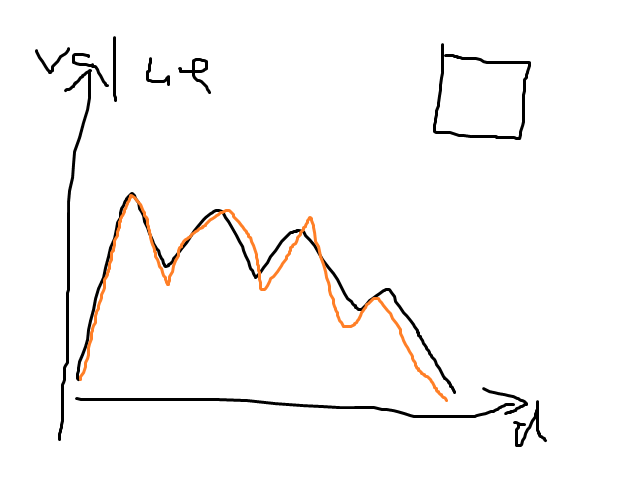
\includegraphics[height=4.5cm]{images/mmd.png}
\caption{One kernel at $x_s$ ({\it dotted kernel}) or two kernels at
$x_i$ and $x_j$ ({\it left and right}) lead to the same summed estimate
at $x_s$. }
\label{fig:example}
\end{figure}

\subsubsection{Unsupervised weights regularizer on Element-wise Multiply Layer}
In works [decaf][][], the last feature vector layer are regarded as the final representation of images. (how to introduce beyond sharing weights) In domain adaptation tasks, when generic deep model are trained with abundant data from source domain, the last element-wise layer mentioned in Sec \ref{section:Element-wise Multiply Layer} also includes rich information leading to the final output. For the nodes in the output layer, inputs from element-wise layers that will contribute to its value are not randomly decided. In this paper, we assume that the distribution of $\vec{m}_{b,o}$ of the last element-wise layer on both source and target domain should be similar. In the last element-wise multiply layer, every dimension of $\vec{m}_{b,o}$ may contribute to the final output. However, as the old model on source domain are trained with abundant images, the distribution of $\vec{m}^{T}_{b,o}$ should be consistent compared with $\vec{m}^{S}_{b,o}$ of source domain when adapting deep network on target domain. We utilize MMD (maximum mean discrepancy) to encode the similarity of element-wise multiply layer of source domain and target domain:
\begin{equation}\label{equation:LMMD}
  L_{MMD}(\theta^{T}|{\bf X}^{S},{\bf X}^{T},\theta^{S}) = \frac{1}{N^{O}} \sum^{N^{O}}_{o=1}{\parallel \frac{1}{N^{B}}\sum^{N^{B}}_{b=1}{\vec{m}^{T}_{b,o}} - \frac{1}{N^{B}}\sum^{N^{B}}_{b=1}{\vec{m}^{S}_{b,o}} {\parallel}^{2}  }
\end{equation}
which can also interpreted as the Euclidean distance between the center of $\vec{m}^{T}_{b,o}$ and $\vec{m}^{S}_{b,o}$ across all output nodes. It's unpractical to get the distribution of the whole training set, while too few images cannot obtain a stable center for regularization. In our experiments, the $L_{MMD}(\cdot)$ loss is calculated for every batch. An example comparison of centers of $\vec{m}^{S}_{b_{i},o}$ and $\vec{m}^{S}_{b_{j},o}$ are shown in Fig x(1).

\begin{figure}
\centering
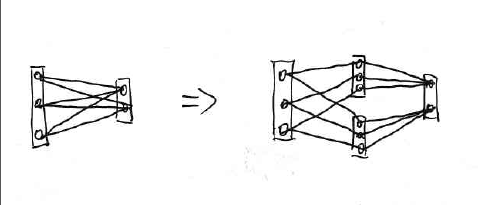
\includegraphics[height=4.5cm]{images/fullconnectlayers.png}
\caption{One kernel at $x_s$ ({\it dotted kernel}) or two kernels at
$x_i$ and $x_j$ ({\it left and right}) lead to the same summed estimate
at $x_s$. }
\label{fig:example}
\end{figure}

\section{Experiment Results}
\label{section:Experiment Results}

In this section, we introduce experiment results on both surveillance applications and standard domain adaptation dataset. Our motivation for unsupervised domain adaptation method is for easier deployment of  We firstly evaluate our approach on video surveillance. Then we employ our approach to standard domain adaptation benchmarks on both supervised and unsupervised settings to demonstrate the effectiveness of our method.

\begin{figure}
\centering
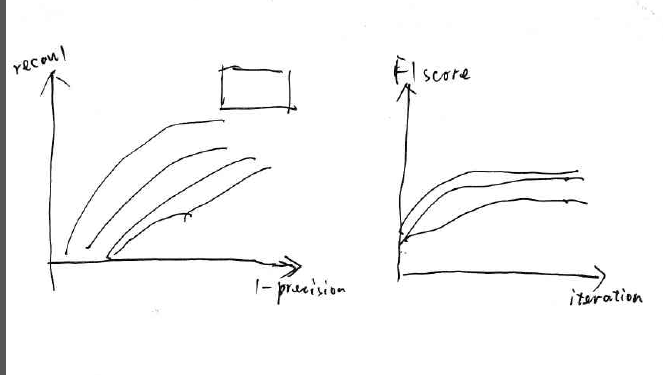
\includegraphics[height=4.5cm]{images/precisionrecall.png}
\caption{One kernel at $x_s$ ({\it dotted kernel}) or two kernels at
$x_i$ and $x_j$ ({\it left and right}) lead to the same summed estimate
at $x_s$. This shows a figure consisting of different types of
lines. Elements of the figure described in the caption should be set in
italics,
in parentheses, as shown in this sample caption. The last
sentence of a figure caption should generally end without a full stop}
\label{fig:example}
\end{figure}

\subsection{Domain Adaptation on Crowd Dataset}

\subsubsection{Dataset and evaluation metrics}
To show the effectiveness of our domain adaptation approach on people detection, we collected a dataset consisting of 3 target scenes for target domain. These three scenes contain 1308, 1213 and 331 un-annotated images with 0000, 0000, 0000 people instances respectively. For each scene, 100 images are annotated for evaluation. Instead of labelling the whole body of a person, we labels the head of a person as bounding box during training. The motivation for labelling only people heads comes from detection of indoor people or in crowded scenes, where the body of a person may be invisible. The dataset for source domain are Brainwash Dataset released on http://d2.mpi-inf.mpg.de/datasets. Brainwash Dataset consists of over 11917 images from 3 crowded scenes. Examples of images from source and target domain are shown in Fig x(!).

Our evaluation metrics for detection uses the protocol defined in PASCAL VOC \cite{everingham2015pascal}. To judge a predicted bounding box whether correctly matches a ground truth bounding box, their intersection over their union must exceed 50\%. And Multiple detections of the same ground truth bounding box are regarded as one correct prediction. We plot the precision-recall curve in Fig x(!). Also, the F1 score $F1 = 2*precision*recall/(precision+recall)$ during the adaptation process are also shown in Fig x(!).



\subsubsection{Experimental settings}
We use deep learning framework Caffe \cite{jia2014caffe} as the adaptation architecture of our approach. During the adaptation, we set learning rate as 0.01 and momentum as 0.5. At initialization stage, GoogLeNet weights are firstly used to initialize source model of source stream, while parameters in RNN layers are randomly initialized from a uniform distribution. For each iteration, 100 auto-annotated images from target domain and 1000 annotated images from source domain are alternatively used for training. The outputs of our detection network contains bounding box locations and corresponding confidence, thus there are two full connected layers between the last feature vector layer and the final outputs. Experiments of unsupervised regularizer on element-wise layer for bounding box regression have no additional improvement on the performance when regularizer on element-wise layer for box confidence classification are added already. Our approach on domain adaptation are executed separately in the 3 target scenes.

\subsubsection{Comparison with baseline methods}
To demonstrate the effectiveness of our approach, 4 methods are compared with method 4 as our final approach:
\begin{enumerate}
\item Only auto-labeled samples on target domain are used for training, and without any unsupervised regularizer.
\item Only auto-labeled samples on target domain are used for training, with MMD regularizer on last element-wise multiply layer as unsupervised weights regularizer.
\item Both auto-labeled images from target domain and labeled images from source domain are alternately sampled for training, with MMD regularizer on last feature vector as unsupervised weights regularizer.
\item Both auto-labeled images from target domain and labeled images from source domain are alternately sampled for training, with MMD regularizer on last element-wise multiply layer as unsupervised weights regularizer.
\end{enumerate}
Fig x(!) plots the precision-recall curve of the above comparison methods in target scene 1). Also, the F1 score changes of every iteration during adaptation process are also depicted in Fig x(!). Table x(!) gives concrete precision and recall value of the 4 comparison methods on three target scenes when the F1 scores are at their highest. Examples of adaptation results are shown in Fig x(!).

\begin{table}
\centering
\begin{tabular}{l  c c c c c c c c c c c}
  \hline
  % after \\: \hline or \cline{col1-col2} \cline{col3-col4} ...
    &   \multicolumn{3}{c}{Scene 1}   & & \multicolumn{3}{c}{Scene 2} & &  \multicolumn{3}{c}{Scene 3}   \\
   \cline{2-4} \cline{6-8} \cline{10-12}
    & ~~1-Pr~~ & ~~Re~~ & ~~F1~~ & & ~~1-Pr~~ & ~~Re~~ & ~~F1~~ & & ~~1-Pr~~ & ~~Re~~ & ~~F1~~\\
  \hline
  method 0~~ & 0.101 & 0.187 & 0.309 & ~~ & 0.015 & 0.683 & 0.807 & ~~ & 0.035 & 0.412 & 0.577 \\
  method 1~~ & 0.245 & 0.408 & 0.530 & ~~ & 0.632 & 0.905 & 0.524 & ~~ & 0.176 & 0.778 & 0.800 \\
  method 2~~ & 0.284 & 0.476 & 0.572 & ~~ & 0.012 & 0.837 & {\bf 0.906} & ~~ & 0.078 & 0.653 & 0.764 \\
  method 3~~ & 0.109 & 0.496 & 0.637 & ~~ & 0.002 & 0.721 & 0.838 & ~~ & 0.044 & 0.611 & 0.746 \\
  method 4~~ & 0.140 & 0.530 & {\bf 0.656} & ~~ & 0.006 & 0.811 & 0.893 & ~~ & 0.097 & 0.778 & {\bf 0.836} \\
  \hline
\end{tabular}
\end{table}

\subsubsection{Performance evaluation}
From the Table x(!) and Fig x(1), we have the following observations:
\begin{itemize}
  \item The recall values of method 1,2,3,4, which all utilized iteration algorithm to upgrade the target model, are larger than that of method 0, which are source model trained on source domain. This implies the effectiveness of our iteration algorithm in auto-annotation and iterative training.
  \item Compared with method 1, method 2 has higher F1 score. Their difference on whether a MMD regularizer are added into loss function demonstrates that our unsupervised regularizer can suppress data error and thus boost the final recall.
  \item Method 4 has both higher precision and higher recall than method 2, which demonstrates the effectiveness of additional samples from source domain during adaptation process.
  \item Compared with method 3, the recall of method 4 are further boosted. This results from the transformed element-wise layer which provided better regularization effect on the target model.
\end{itemize}



\subsection{Domain Adaptation on Standard Classification Benchmark}

\subsubsection{Office dataset}
The Office dataset \cite{saenko2010adapting} comprises 31 categories of objects from 3 domains (Amazon, DSLR, Webcam). Example images are depicted in Fig. x(!). As Amazon domain contains 2817 labelled images, which is the largest, we take it as source domain and Webcam domain as target domain. We follow the standard protocol for both supervised and unsupervised settings. Specifically, for supervised domain adaptation, we use 20 randomly sampled images with labels for each category as training data for Amazon domain. When evaluate on unsupervised domain adaptation, 3 labelled images from target domain are additional selected for each class. For both settings, the rest of images on target domain are used for evaluation.

\begin{figure}
\centering
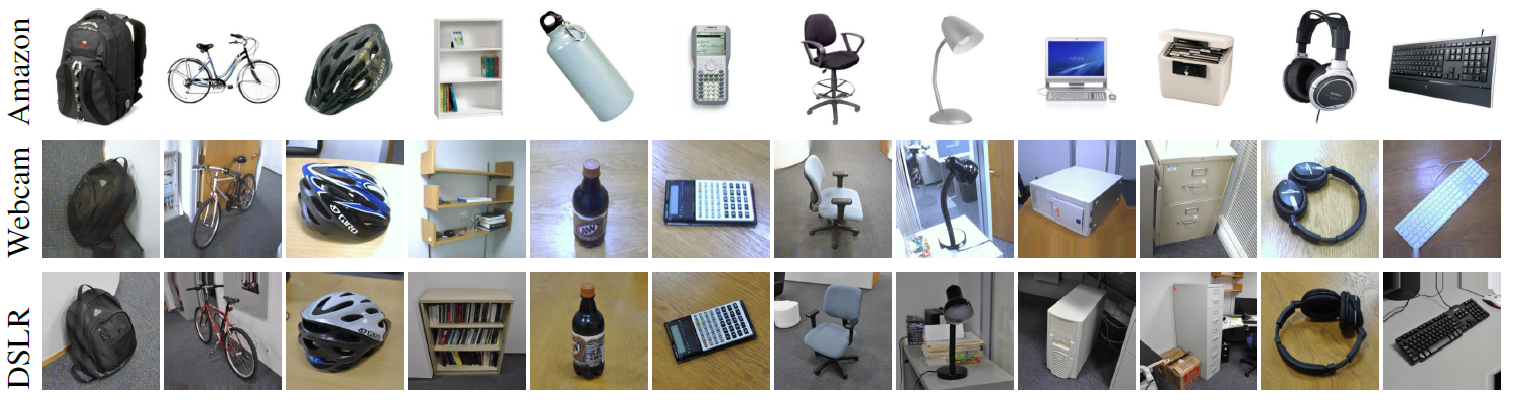
\includegraphics[height=4cm]{images/officeimages.png}
\caption{One kernel at $x_s$ ({\it dotted kernel}) or two kernels at
$x_i$ and $x_j$ ({\it left and right}) }
\label{fig:example}
\end{figure}

\subsubsection{Experimental settings and network design}
On supervised setting, we reused the architecture in people detection. We utilize AlexNet \cite{krizhevsky2012imagenet} as the generic model of both streams. Firstly, we train the source model on source stream with provided training data from Amazon domain. Then iteration algorithm mentioned in Sec \ref{Section:Iterative Algorithm} are utilized for adaptation. The auto-labelling tool takes images on target domain with confidence exceeding 0.9 as training data for next iteration. The difference is besides auto-labelled images on target domain, 3 human labelled images for each class are also included as training data for target model. For each iteration, 100 images are randomly sampled from training data. The unsupervised MMD regularizer added on the element-wise layer transformed from the last full connect layer of target model set the coefficient value $\alpha$ as 10 on Eq \ref{Eq:lmmd}, the same as that in people detection task.

We use the same experimental setting for our unsupervised adaptation, except that at adaptation stage, no human labelled images can be added into the training set.
\subsubsection{Performance evaluation}
In Table x(!), we compare our approach with other six recently published works in both supervised and unsupervised settings. The outstanding performance on both settings confirms the effectiveness of our iteration algorithm and MMD regularizer on the element-wise layer transformed from the last full connect layer.


\begin{table}
\centering
\begin{tabular}{l c c}
  \hline
  % after \\: \hline or \cline{col1-col2} \cline{col3-col4} ...
   & \multicolumn{2}{c}{A $\rightarrow$ W}    \\
   \cline{2-3}
   ~~~~~~~~~~~~~~~~~~~~~~~~~~~~~~~
   ~~~~~~~~~~~~~~~~~~~~~~~~~~~~~~~
    & ~Supervised~ & ~Unsupervised~ \\
  \hline
  GFK(PLS,PCA)\cite{gong2012geodesic} & 46.4 & 15.0 \\
  SA \cite{fernando2013unsupervised} & 45.0 & 15.3 \\
  DA-NBNN \cite{tommasi2013frustratingly} & 52.8 & 23.3 \\
  DLID \cite{chopra2013dlid}& 51.9 & 26.1 \\
  DeCAF${}_{6}$S \cite{donahue2013decaf} & 80.7 & 52.2 \\
  DaNN \cite{ghifary2014domain}& 53.6 & 35.0 \\
  \hline
  Ours & {\bf 84.3} & {\bf 66.3} \\
  \hline
\end{tabular}
\end{table}


\section{Conclusions}
\label{section:Conclusions}

The paper ends with a conclusion.

\begin{figure}
\centering
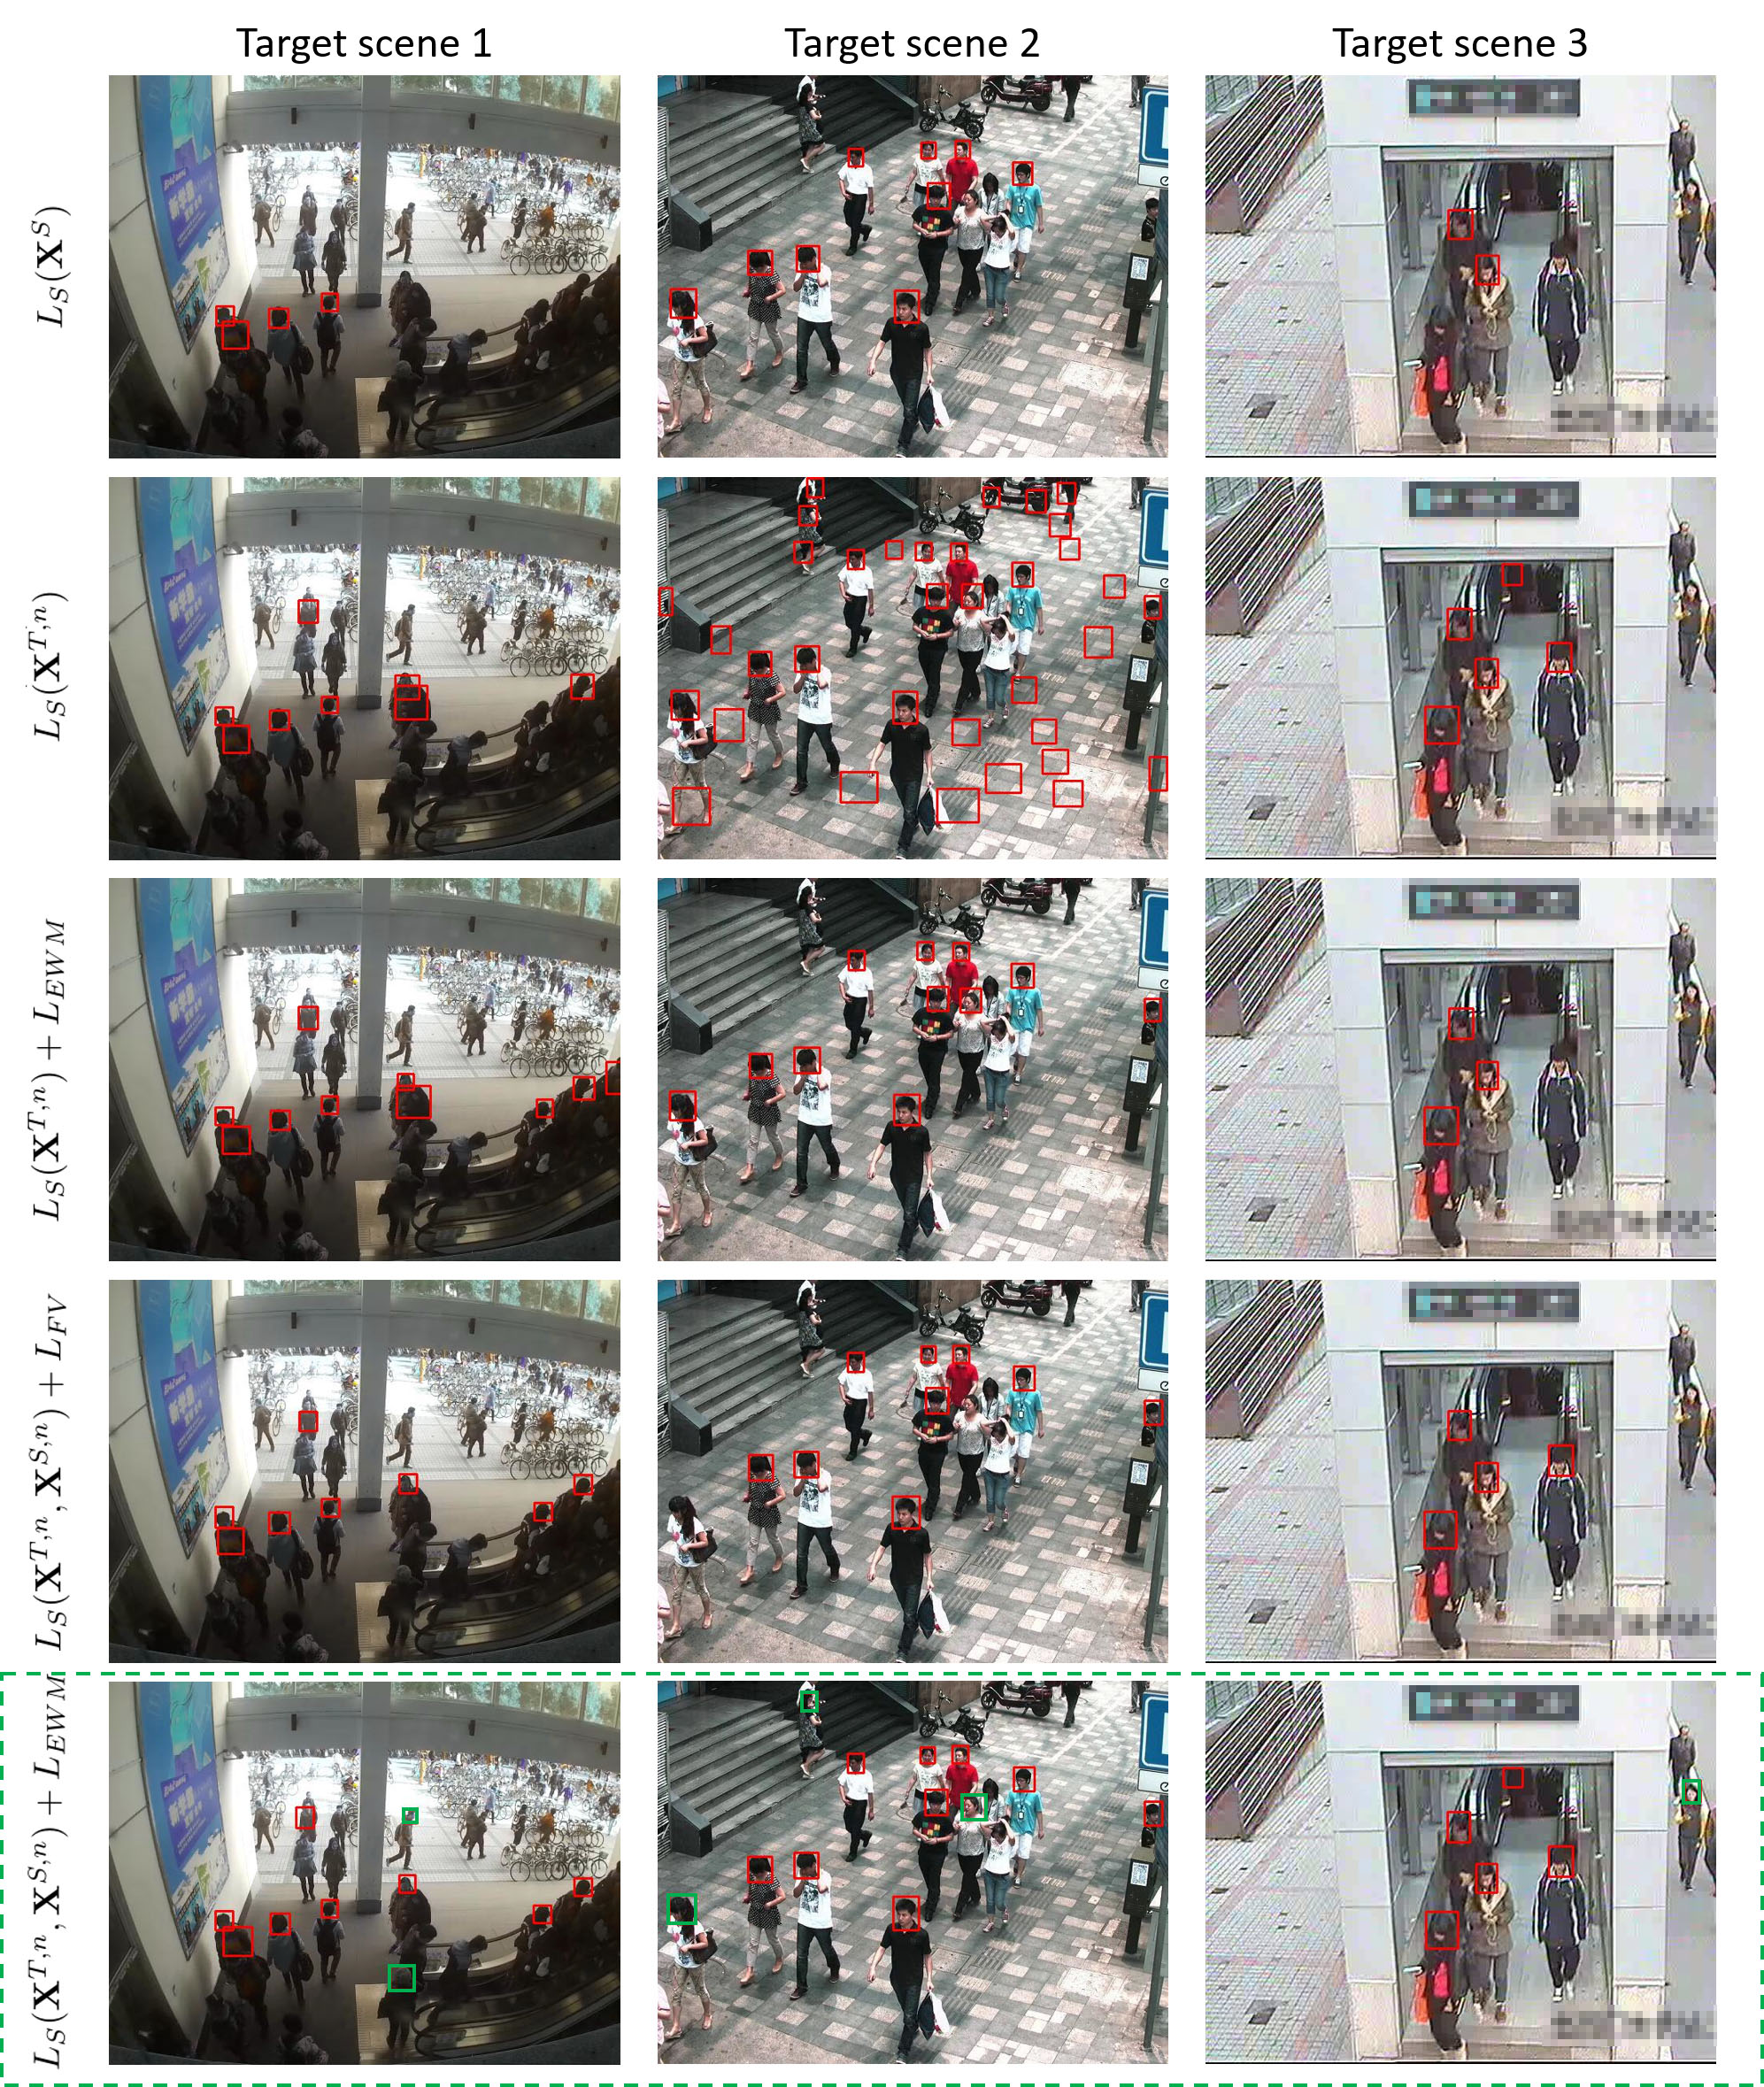
\includegraphics[height=13cm]{images/detectionresult.png}
\caption{One kernel at $x_s$ ({\it dotted kernel}) or two kernels at
$x_i$ and $x_j$ ({\it left and right}) }
\label{fig:example}
\end{figure}

\bibliographystyle{splncs}
\bibliography{egbib}
\end{document}
